\documentclass[bachelor, och, pract]{SCWorks}
% параметр - тип обучения - одно из значений:
%    spec     - специальность
%    bachelor - бакалавриат (по умолчанию)
%    master   - магистратура
% параметр - форма обучения - одно из значений:
%    och   - очное (по умолчанию)
%    zaoch - заочное
% параметр - тип работы - одно из значений:
%    referat    - реферат
%    coursework - курсовая работа (по умолчанию)
%    diploma    - дипломная работа
%    pract      - отчет по практике
%    pract      - отчет о научно-исследовательской работе
%    autoref    - автореферат выпускной работы
%    assignment - задание на выпускную квалификационную работу
%    review     - отзыв руководителя
%    critique   - рецензия на выпускную работу
% параметр - включение шрифта
%    times    - включение шрифта Times New Roman (если установлен)
%               по умолчанию выключен
\usepackage[T2A]{fontenc}
\usepackage[utf8]{inputenc}
\usepackage[english,russian]{babel}
\usepackage{graphicx}
\usepackage[sort,compress]{cite}
\usepackage{amsmath}
\usepackage{amssymb}
\usepackage{amsthm}
\usepackage{fancyvrb}
\usepackage{longtable}
\usepackage{array}
\usepackage{minted}
\usepackage{tempora}
\usepackage[hidelinks]{hyperref}
% % При использовании biblatex вместо bibtex
%\usepackage[style=gost-numeric]{biblatex}
%\addbibresource{thesis.bib}

\begin{document}

% Кафедра (в родительном падеже)
\chair{информатики и программирования}

% Тема работы
\title{Разработка древовидной иерархии модулей управления компонентами ALT Linux}

% Курс
\course{4}

% Группа
\group{441}

% Факультет (в родительном падеже) (по умолчанию "факультета КНиИТ")
%\department{факультета КНиИТ}

% Специальность/направление код - наименование
%\napravlenie{02.03.02 "---- Фундаментальная информатика и информационные технологии}
\napravlenie{02.03.03 "---- Математическое обеспечение и администрирование информационных систем}
%\napravlenie{09.03.01 "---- Информатика и вычислительная техника}
%\napravlenie{09.03.04 "---- Программная инженерия}
%\napravlenie{10.05.01 "---- Компьютерная безопасность}

% Для студентки. Для работы студента следующая команда не нужна.
%\studenttitle{Студентки}

% Фамилия, имя, отчество в родительном падеже
\author{Шарова Кирилла Владимировича}

% Заведующий кафедрой
\chtitle{доцент, к.\,ф.-м.\,н.} % степень, звание
\chname{М.\,В.\,Огнева}

%Научный руководитель (для реферата преподаватель проверяющий работу)
\satitle{доцент, к.\,ф.-м.\,н.} %должность, степень, звание
\saname{М.\,В.\,Огнева}

% Руководитель практики от организации (только для практики,
% для остальных типов работ не используется)

\patitle{Заместитель генерального директора}
\patitlecompany{ООО <<Базальт СПО>>}
\paname{Е.\,А.\,Синельников}

% Семестр (только для практики, для остальных
% типов работ не используется)
\scourse{3}
\term{6}

% Наименование практики (только для практики, для остальных
% типов работ не используется)
\practtype{производственная}

% Продолжительность практики (количество недель) (только для практики,
% для остальных типов работ не используется)
\duration{4}

% Даты начала и окончания практики (только для практики, для остальных
% типов работ не используется)
\practStart{22.06.2024}
\practFinish{19.07.2024}

% Год выполнения отчета
\date{2024}

\maketitle

% Включение нумерации рисунков, формул и таблиц по разделам
% (по умолчанию - нумерация сквозная)
% (допускается оба вида нумерации)
%\secNumbering


\tableofcontents

% Раздел "Обозначения и сокращения". Может отсутствовать в работе
% \abbreviations
% \begin{description}
%     \item ... "---- ...
%     \item ... "---- ...
% \end{description}

% Раздел "Определения". Может отсутствовать в работе
%\definitions

% Раздел "Определения, обозначения и сокращения". Может отсутствовать в работе.
% Если присутствует, то заменяет собой разделы "Обозначения и сокращения" и "Определения"
%\defabbr


% Раздел "Введение"

\intro

ALT Linux --- это семейство российских дистрибутивов Linux, разрабатываемых компанией <<Базальт СПО>>.
Они предназначены для использования в государственных учреждениях, образовательных организациях и других структурах, где требуется надёжное и безопасное программное обеспечение.

Одной из особенностей ALT Linux является его ориентация на безопасность и защиту информации.
В дистрибутивы включены инструменты для шифрования данных, защиты от вирусов и несанкционированного доступа.
Также ALT Linux поддерживает работу с отечественными криптографическими алгоритмами и средствами аутентификации.

Компания <<Базальт СПО>> предоставляет техническую поддержку и обновления для ALT Linux, что обеспечивает его надёжность и стабильность.
Разработчики также проводят обучение и консультации по использованию системы, что способствует её распространению и внедрению.

В целом, ALT Linux представляет собой надёжную и безопасную операционную систему (далее ОС), которая может быть использована в различных областях деятельности.
Она позволяет снизить зависимость от иностранных поставщиков программного обеспечения и обеспечить безопасность информационных систем\cite{a_basealt}, % ссылка-заглушка пока что
что соответствует текущей государственной политике импортозамещения.

Целью работы является разработка древовидной иерархии модулей управления компонентами ОС ALT Linux.

Поставленная цель определила следующие задачи.
\begin{itemize}
    \item Научиться собирать RPM-пакеты инструментами ALT Linux.
    \item Начать прохождение процедуры Join.
    \item Изучить систему межпроцессного взаимодействия D-Bus.
    \item Научиться разрабатывать и пакетировать приложения на C++ и Qt5.
    \item Реализовать древовидную иерархию компонентов в alterator-application-components.
\end{itemize}

\section{Программы и их хранение в ALT Linux} % Объединение первых трех задач, формально теоретический раздел

\subsection{RPM-пакеты и средства пакетизации ALT Linux}

\textit{RPM-пакеты}

Неотъемлемой частью дистрибутивов Linux являются хранилища программного обеспечения (далее ПО), которые зачастую являются собственными и индивидуальными для конкретного дистрибутива.
Такое хранилище ПО называется репозиторием пакетов Linux.
В общем случае пакеты содержат директории с файлами, метаданными и информацией о зависимостях для их установки.
Репозитории пакетов Linux предназначены для стандартизации процесса установки ПО из удалённого хранилища, что предоставляет удобство как разработчикам, так и пользователям.

Самыми популярными форматами таких пакетов являются DEB (свойственны Debian-подобным дистрибутивам) и RPM (Red Hat Package Manager).
Репозитории пакетов семейства дистрибутивов ALT Linux основаны на пакетах RPM.

RPM-пакетизация состоит из следующих этапов.
\begin{itemize}                                                                           
    \item Нахождение исходного текста программы (опционально).                           
    \item Написание инструкции сборки пакета.                                              
    \item Непосредственная сборка пакета.                            
\end{itemize}

Исходный текст программы часто можно получить на официальном сайте или странице программы.
Исходный текст может быть в виде tar-архива, git-репозитория и т.п.
Также альтернативным источником исходного текста может быть пакет формата src.rpm или deb-src (у Debian-подобных дистрибутивов)\cite{a_rpm}.

В качестве сценария для сборки выступает файл формата spec (далее SPEC-файл).
Структура SPEC-файла следующая.
\begin{itemize}                                                                           
    \item Шапка с информацией о пакете.                          
    \item Описание пакета.              
    \item Секция предварительной обработки исходных данных.
    \item Секция сборки исходного текста.
    \item Секция установки результата сборки.
    \item Секция файлов.
    \item Секция метаданных о журнале изменений версий пакета.
\end{itemize}

В общем случае шапка SPEC-файла содержит следующую информацию.
\begin{itemize}                                                                                      
    \item Название пакета (Name).                                                              
    \item Версия ПО, включенного в пакет (Version).                                                                           
    \item Версия пакета (Release).                                          
    \item Резюме ПО (Summary).                                                            
    \item Лицензия распространения ПО (License).                   
    \item Категория, к которой относится ПО (Group).
    \item Электронный ресурс ПО (URL). 
    \item Имена архивов с исходными текстами (Source).
    \item Имена файлов исправлений (патчей), применяемых к исходным текстам (Patch).
    \item Архитектуры процессоров, на которых собирается пакет (BuildArch).
    \item Требуемые пакеты для сборки (BuildRequires).
    \item Требумые пакеты для запуска (Requires).
\end{itemize}

Секция предварительной обработки исходных данных (\%prep) включает в себя распаковку архива с исходниками в директорию сборки с установкой соответствующих пользовательских прав доступа.
Также при необходимости накладываются патчи, перечисленные в шапке под соответствующим ключом (например, макрос \%patch0 разворачивается в установку первого патча из перечисления).

Секция сборки исходного текста (\%build) включает в себя инструкции для непосредственной сборки предварительно обработанных исходных текстов в директории сборки.

Результат работы сборки проходит следующий этап в секции (\%install) с установкой собранного ПО в локальный корневой каталог пакета с настройкой пользовательских прав доступа.

Секция файлов (\%files) содержит перечисление файлов, полученных в результате сборки и установки в локальный корневой каталог, которые устанавливаются в пользовательскую систему при установке пакета.

Секция журнала изменений (\%changelog) включает в себя историю релизов пакета\cite{a_rpm-macro}.

Сборка RPM-пакета происходит в директории, содержащей, в общем случае, архив с исходными текстами программы, а также SPEC-файл.
Классическая сборка RPM-пакета из исходных текстов происходит посредством вызова следующей команды:

\begin{Verbatim}
$ rpmbuild -ba имя_SPEC-файла.spec
\end{Verbatim}

\textit{Средства пакетизации ALT Linux}

Дистрибутивы ALT Linux предоставляют инструменты собственной разработки для более надёжной и удобной в большинстве случаев сборки RPM-пакетов.

Например, классическая сборка RPM-пакета опирается на уже предустановленные в системе требуемые зависимости.
В процессе написания SPEC-файла можно забыть про некоторые требуемые зависимости для сборки, которые уже содержатся в системе.
Также требуемые зависимости для сборки могут быть специфичными для сборки конкретных исходных файлов и быть нужными только непосредственно при сборке.
Для того, чтобы решить проблему в точности требуемых пакетов и остаточных пакетов после процесса сборки необходимо производить сборку в <<чистой>> временной системе.

Такую систему эмулирует Hasher --- собственная разработка ALT Linux.
Hasher создает "чистую" и контролирумую среду внутри ОС, в которой производится сборка RPM-пакета.
Изолированность среды сборки позволяет вне зависимости от конфигурации системы пользователя повторить результат сборки RPM-пакета на другом компьютере и для любой из веток репозитория (подробнее в 1.2).

Сборка при помощи Hasher происходит от обычного пользователя, добавленного с помощью hasher-useradd (подробнее про настройку Hasher в 2.1):

\begin{Verbatim}
$ hsh ~/hasher имя_архива.src.rpm
\end{Verbatim}

Где ~/hasher --- директория, в которой строится сборочная среда (chroot). Рекомендуется это делать внутри домашней директории\cite{a_hasher}.

Также для ALT Linux был разработан инструмент Gear, который делает процесс сборки пакетов из исходных файлов более удобным. 
Например, очень часто исходные тексты ПО содержатся в Git-репозиториях.
Таким образом, Gear позволяет собирать RPM-пакеты напрямую из склонированного Git-репозитория, являясь, грубо говоря, более высокоуровневой надстройкой над rpmbuild с использованием Git.

Gear-репозиторий --- это Git-репозиторий, содержащий SPEC-файл и инструкцию архивации в .gear/rules, которая, чаще всего, содержит:
\begin{Verbatim}
tar: .
\end{Verbatim}

Что означает упаковку в tar-архив данных, содержащихся в текущей директории.
Причем архивация происходит не столько из исходных файлов репозитория, сколько из истории Git-репозитория. 
Поэтому все изменения в Gear-репозитории необходимо сохранять в истории (команда git commit содержимого git-индекса).

Сборка при помощи Gear происходит посредством вызова следующей команды (находясь в директории Gear-репозитория):
\begin{Verbatim}
$ gear-rpm -ba
\end{Verbatim}

SPEC-файл в таком случае не требуется передавать в качестве аргумента явно, так как он будет найден в истории Git\cite{a_gear}.

Однако и Gear, и Hasher могут быть использованы вместе, что даёт удобную, надёжную и <<чистую>> сборку RPM-пакета.
И производится это при помощи следующей команды (находясь в директории Gear-репозитория):

\begin{Verbatim}
$ gear-hsh
\end{Verbatim}

\subsection{Проект <<Сизиф>> и процедура Join}

Как было упомянуто ранее, пакеты ПО хранятся в специальных для конкретного дистрибутива репозиториях.
По специфике релизов ПО отличают 2 вида репозиториев: Rolling Release и Fixed Release.

Rolling Release (рус. скользящий выпуск) --- вид постоянно обновляемых репозиториев.
Такие репозитории содержат, как правило, пакеты с наиболее актуальными версиями ПО.
Частота обновления Rolling Release репозиториев связана с отсутствием как таковой процедуры тестирования пакетов ПО.
Резюмируя, такой подход обеспечивает пользователя пакетами с актуальными версиями ПО, однако не гарантируется стабильность пользовательского опыта.

Fixed Release (рус. постоянный, неизменный выпуск) репозитории имеют достоинства в виде стабильности включаемых пакетов.
Для попадания туда пакеты из, как правило, Rolling Release репозиториев проходят тщательное тестирование.
В противоположность Rolling Release, это обеспечивает стабильность пользовательского опыта, однако такой подход имеет недостаток в виде частоты выпуска стабильных веток.
Так как стабильные ветки обновляются не так часто, чаще всего они содержат устаревшие версии ПО.

В семействе дистрибутивов ALT Linux выделены следующие основные стабильные ветки APT-репозитория, на которых базируются непосредственно дистрибутивы: p5, p6, p7, p8, p9 и p10.
Также есть ветки сообщества: 5.1, t6, t7. Номер релиза сборки дистрибутива соответствует номеру ветки.
Например, ALT Workstation 10 базируется на ветке p10.

ALT Linux помимо стабильных веток обладает ключевой особенностью: проект <<Sisyphus>>.
Sisyphus или же <<Сизиф>> является одним из крупнейших репозиториев свободного ПО в мире.
Целью проекта является развитие репозитория свободного ПО для разработки на его основе дистрибутивов и других решений.
Если репозитории, маркированные \textit{p}, разрабатываются непосредственно сотрудниками Базальт СПО, то <<Сизиф>> представляет собой инфраструктуру разработки,
регулярно обновляемую и поддерживаемую сообществом ALT Linux Team\cite{a_sisyphus}.

По сути Sisyphus является Rolling Release репозиторием, на базе которого уже разрабатываются Fixed Release репозитории.
Кратко говоря, пакеты Sisyphus, прошедшие процедуру проверки, попадают в стабильную ветку.
Участники сообщества ALT Linux Team также могут оставлять запрос на вхождение их пакета в стабильный релиз, проходя для этого некоторую процедуру.
Также на основе Sisyphus существуют неофициальные сборки дистрибутивов, которые используются, как правило, разработчиками сообщества ALT Linux Team.

Чтобы стать разработчиком проекта <<Сизиф>>, необходимо присоединиться к сообществу ALT Linux Team, пройдя процедуру под названием <<Join>>. 
Для того, чтобы новый человек стал частью команды, создаётся специальная группа из заинтересованных участников.

В эту группу, как правило, входят следующие лица:
\begin{itemize}
    \item секретарь команды, который следит за этапами процесса и выполняет административные задачи;
    \item ментор, помогающий новичку адаптироваться, отвечающий на его вопросы и принимающий решение о готовности кандидата;
    \item рецензент работы, который проводит независимую оценку готовности новичка по результатам его работы и подтверждает его готовность.
\end{itemize}
Четвёртым участником является сам кандидат.

Необходимыми навыками для вступления в ALT Linux Team являются:
\begin{itemize}
    \item умение собирать ПО из исходных текстов;
    \item навыки чтения, правки и написания SPEC-файлов;
    \item знание специфики пакетирования RPM под ALT Linux.
\end{itemize}

По итогу прохождения процедуры Join кандидату даётся SSH-доступ к git.alt и gyle.alt (сборочнице), и вместе с тем возможность выкладывать пакеты в репозиторий ALT.
Единственной обязанностью члена ALT Linux Team является хранение ключей подписи (SSH и GPG) в недоступном для других людей месте\cite{a_join}.

\subsection{Системы межпроцессного взаимодействия}

Коммуникация сущностей является неотъемлемой частью любой ОС.
Встречаются следующие виды взаимодействий:

\begin{itemize}
    \item межпотоковое взаимодействие (Inter-Thread Communication);
    \item межпрограммное взаимодействие (Inter-Application Communcation);
    \item межпроцессное взаимодействие (Inter-Process Communcation).
\end{itemize}

Коммуникация между потоками, программами и процессами инкапсулирована в самом ядре ОС, поэтому доступ к ней осуществляется при помощи низкоуровневых библиотек или библиотек, основанных на низкоуровневых компонентах.

В частности, нас интересует межпроцессное взаимодействие. Дадим определение термину <<процесс>>.

Процесс --- это среда выполнения для работы экземпляра программы, порождённая ОС, а точнее --- планировщиком, в виртуальном адресном пространстве.
К примеру, при запуске какой-либо программы создается процесс под неё, которому выделяется часть оперативной памяти.
В рамках которой, зачастую, и производится исполнение этой самой программы, не считая запрос динамической памяти к ОС.
Этот процесс наделяется некоторыми свойствами, также ему присваивается уникальный идентификатор.

Как известно, в ОС может существовать множество процессов.
Процессор обрабатывает эти процессы не одновременно.
За счёт вышеупомянутого планировщика он очень быстро переключается с одного процесса на другой, поэтому может казаться, что процессы выполняются независимо и параллельно.
А значит создаётся ощущение многозадачности.

Одной из систем межпроцессного взаимодействия (IPC) является D-Bus.
D-Bus --- это система для межпроцессного взаимодействия (IPC). Архитектурно она состоит из нескольких уровней.

\begin{itemize}
    \item Библиотека, libdbus, которая позволяет двум приложениям подключаться друг к другу и обмениваться сообщениями.
    \item Исполняемый файл демона (фоновой утилиты) шины сообщений, построенный на libdbus, к которому могут подключаться несколько приложений.
        Демон может направлять сообщения от одного приложения к нулю или нескольким другим приложениям.
    \item Библиотеки-оболочки или привязки, основанные на конкретных фреймворках приложений.
        Например, libdbus-glib и libdbus=qt. Существуют также привязки к таким языкам, как Python.
        Эти библиотеки-оболочки - это API, которые следует использовать большинству людей, поскольку они упрощают детали программирования на D-Bus.
        libdbus задуман как низкоуровневый сервер для привязок более высокого уровня.
        Большая часть API libdbus полезна только для реализации привязки.
\end{itemize}

libdbus поддерживает только соединения <<один к одному>>, как и обычный сетевой сокет.
Однако вместо отправки потоков байтов по соединению вы отправляете сообщения.
Сообщения имеют заголовок, определяющий тип сообщения, и тело, содержащее полезную нагрузку данных.
libdbus также абстрагирует используемые точки соединения (сокеты или что-либо еще) и обрабатывает такие детали, как аутентификация.

Демон шины сообщений является маршрутизатором, который содержит соединения <<один к одному>> с приложениями, использующими libdbus.
Приложение отправляет сообщение демону шины, а демон шины пересылает сообщение другим подключенным приложениям по мере необходимости.

Демон шины имеет несколько экземпляров на обычном компьютере.
Первый экземпляр --- это машинно-глобальный singleton (объект класса в единственном экземпляре), то есть системный демон, подобный sendmail или Apache.
Этот экземпляр имеет строгие ограничения безопасности на то, какие сообщения он будет принимать, и используется для общесистемной связи.
Другие экземпляры создаются по одному на сеанс входа пользователя в систему.
Эти экземпляры позволяют приложениям в сеансе пользователя взаимодействовать друг с другом.

Общесистемные демоны и демоны для каждого пользователя разделены.
Обычный межсессионный IPC не включает процесс общесистемной шины сообщений и наоборот.

Протокол D-Bus оперирует такими сущностями как объект.
API libdbus предоставляет концепцию, называемую путём к объекту.
Идея пути к объекту заключается в том, что привязки более высокого уровня могут называть собственные экземпляры объектов и позволять удаленным приложениям ссылаться на них.

Объекты содержат в себе члены, называемые методами и сигналами.
Методы --- это операции с некоторыми параметрами (аргументами метода) и возвращаемым значением, которые могут быть вызваны над объектом.
Сигналы передаются с объекта любым заинтересованным наблюдателям этого объекта.
Сигналы могут содержать некоторые полезные данные. Можно сказать, что сообщение в сессии IPC является параметризованным запросом.

Каждый объект поддерживает один или несколько интерфейсов, которые зачастую представляют группы одинаково именованных методов и сигналов.
С помощью интерфейса можно обратиться к конкретной реализации той или иной операции, того или иного сигнала.
Таким образом, интерфейс является <<прослойкой>> между объектом и членом\cite{a_dbus}.

Целевой проект данной работы  <<alterator-application-components>> использует технологию D-Bus, чтобы получать информацию об установленных в системе пакетах для последующей её обработки (подробнее о которой в разделе 2).

\newpage

\section{Разработка системы конфигурации операционной системы ALT Linux}

\subsection{Инструментарий для разработки и пакетизации}

Основная кодовая база проекта alterator-application-components использует язык программирования С++ и фреймворк Qt.
В качестве стандарта языка в ходе работы был выбран С++17 из-за его повсеместной поддержки любыми компиляторами.

Qt --- это кроссплатформенный фреймворк, который предоставляет набор инструментов для создания графических интерфейсов пользователя (GUI), работы с сетью, базами данных и другими задачами разработки.
Он имеет большое сообщество разработчиков и множество готовых компонентов, что упрощает процесс разработки\cite{a_qt}.

В качестве инструментария для взаимодействия между компонентами системы используется модуль Qt D-Bus.
Он позволяет компонентам обмениваться данными и событиями через систему межпроцессного взаимодействия D-Bus.
Это обеспечивает гибкость и масштабируемость системы.

Таким образом, выбор C++ Qt и Qt D-Bus в качестве инструментария разработки обеспечивает высокую производительность, гибкость и надёжность разрабатываемой системы.
Эти инструменты позволяют эффективно решать задачи разработки и обеспечивают лёгкость в поддержке и дальнейшем развитии проекта.

Для сборки исходных текстов в проекте используется кроссплатформенная система сборки CMake.

Все релизы проекта Alterator в первую очередь попадают в репозиторий RPM-пакетов ALT Linux Sisyphus.
Для того, чтобы сборочница на сервере могла создать пакет с бинарными файлами, необходимо иметь исходные тексты проекта, а также SPEC-файл, оформленные в Gear-репозиторий.

Например, возвращаясь к процедуре Join, для её прохождения в качестве проекта для RPM-пакетизации нами была выбрана разработка языка программирования Standard ML of New Jersey\cite{a_smlnj}.
Его SPEC-файл представлен в приложении \ref{spec}.

В файле .gear/rules описаны инструкции по архивации исходных текстов и по поиску файла исправлений (патча) к ним.

\begin{Verbatim}
tar: .
spec: .gear/smlnj.spec
copy?: .gear/*.patch
\end{Verbatim}

В данном случае потребовалось сделать патч из-за ошибки разработчиков в указании флагов для компилятора g++.
Файл патча является текстовым файлом и представлен он в приложении \ref{patch}.

В частном случае подготовка исходных текстов к пакетизации выглядит подобным образом.
После проверки корректности сборки утилитой Hasher в связке с Gear можно отправлять репозиторий в сборочницу.

\subsection{Реализация иерархии компонентов alterator-application-components}

Проект alterator-application-components является частью проекта Alterator.
Он представляет собой конфигуратор ОС семейства ALT Linux.
Данный конфигуратор позволяет пользователям управлять установкой и удалением компонентов, которыми являются группы пакетов, в совокупности выполняющих определённые задачи.

Это ПО по большей части предназначено для системных администраторов.
Решение, основанное на D-Bus, позволяет не только получать данные о пакетах, но и удалённо администрировать серверы.

У компонентов, как правило, есть категория, к которым они относятся.
То есть, отдельно взятые компоненты можно обобщить в единый класс, как, например, <<Система>>.

Однако существующее решение рассчитано только на возможность категоризовать компоненты на 1 уровень вложенности.
Данное ограничение установлено в связи с тем, что решение построения модели (дерева категорий и компонентов) основано на квадратичных циклах.
То есть невозможна такая иерархия категорий и компонентов, при которой у каждой категории может быть родительская категория, кроме тех категорий, которые находятся на верхнем уровне иерархии.

В данной работе было реализовано решение поставленной проблемы с изменением логики построения модели с квадратичных циклов на рекурсивную природу.

Элементарными сущностями в решении являются ComponentCategory и ComponentObject, которые содержат информацию о категории и о компоненте соответственно.
Обе эти сущности обладают некоторыми общими свойствами, поэтому они являются наследниками абстрактного класса AMCObject.

\begin{figure}[!ht]
	\centering
	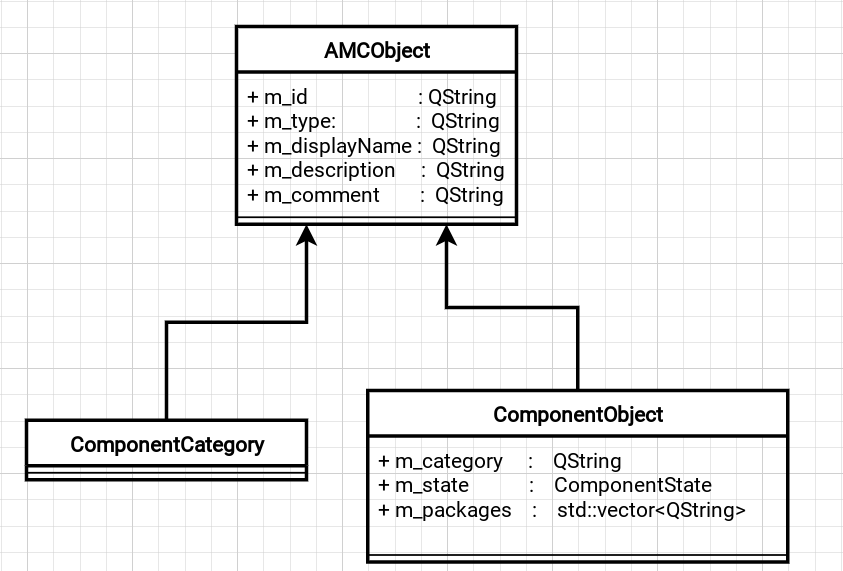
\includegraphics[width=10cm]{amcobject.png}
	\caption{\label{fig:f3}%
	Иерархия наследников AMCObject}
\end{figure}

Для начала, чтобы решить поставленную проблему, потребовалось вынести поле m\_category в родительский класс.
Теперь, когда мы стали полагать, что категория может иметь родительскую категорию, необходимо было изменить процесс построения модели на рекурсивный.
Старая версия метода построения модели представлена в приложении \ref{oldbuild}.

В данной реализации сначала строится список категорий и компонентов посредством вызовов методов buildCategories и buildObjects, где инкапсулировано общение с D-Bus.
Далее в цикле по всем категориям создаётся соответствующая сущность элемента модели (нода дерева) categoryItem, после чего совершается цикл перебора компонентов на поиск тех, которые соответствуют категории на текущей итерации.
Затем, при нахождении искомых компонентов, на ноду вешаются ноды-потомки componentItem.
Такие компоненты извлекаются из списка.
Также в цикле содержится проверка на отсутствие детей у ноды категории, чтобы не добавлять в модель ноды пустых категорий.
Оставшиеся компоненты, которые не были отнесены ни к одной из категории в списке, заносятся в категорию по умолчанию.

Теперь данный метод выглядит образом, представленным в приложении \ref{newbuild}.

Теперь категории и объекты строятся изначально в структуру данных вида словаря, где ключом является ID категории, а значением --- список дочерних категорий или список дочерних объектов соответственно.
В цикле идёт проход по всем категориям, у которых отсутствует родительская категория (ключ --- пустая строка).
Далее аналогичным образом инициализируется нода категории, после чего происходит заход в метод buildInner по созданной ноде.
Метод buildInner является рекурсивным, где из принимаемой ноды считывается ID категории для поиска дочерних категорий/объектов по аналогии с циклом в build.
Выглядит buildInner следующим образом.

\begin{Verbatim}[fontsize=\small,breaklines=true,numbers=left]
void ModelBuilder::buildInner(ModelItem *item,
                              std::unordered_map<QString, std::vector<std::unique_ptr<ComponentCategory>>> &categories,
                              std::unordered_map<QString, std::vector<std::unique_ptr<ComponentObject>>> &components) {
    const QString& parentId = item->data().value<ComponentCategory *>()->m_id;    
    for (auto &category : categories[parentId]) {
        auto categoryItem = std::make_unique<ModelItem>(std::move(category));
        buildInner(dynamic_cast<ModelItem *>(categoryItem.get()), categories, components);
        if (categoryItem->rowCount()) 
            item->insertRow(item->rowCount(), categoryItem.release());
    }
    for (auto& component : components[parentId]) {
        auto componentItem = std::make_unique<ModelItem>(std::move(component));
        item->insertRow(item->rowCount(), componentItem.release());
    }
}
\end{Verbatim}

Условием выхода из рекурсии является пустой список дочерних категорий.

Для того, чтобы с построенной моделью можно было корректно работать, а именно получать её состояние, а также изменять его различными событиями, соответствующие методы также необходимо было переписать.

Компонент принимает одно из трёх состояний:

\begin{itemize}
    \item не установлен;
    \item частично установлен;
    \item установлен.
\end{itemize}

Метод getCurrentState получения текущего состояния всех компонентов модели выглядел следующим образом.

\begin{Verbatim}[fontsize=\small,breaklines=true,numbers=left]
ComponentsState Model::getCurrentState() {
    ComponentsState state{};
    for (int i = 0; i < rowCount(); i++) {
        auto categoryItem = dynamic_cast<ModelItem *>(invisibleRootItem()->child(i));
        for (int j = 0; j < categoryItem->rowCount(); j++) {
            auto componentItem = dynamic_cast<ModelItem *>(categoryItem->child(j));
            auto component = componentItem->data().value<ComponentObject *>();
            if (component)
                state.insert(component->m_id, component->m_state);
        }
    }
    return state;
}
\end{Verbatim}

После переработки он принял следующий вид.

\begin{Verbatim}[fontsize=\small,breaklines=true,numbers=left]
ComponentsState Model::getCurrentState() {
    ComponentsState state{};
    for (size_t i = 0; i < rowCount(); ++i) {
        auto categoryItem = dynamic_cast<ModelItem *>(invisibleRootItem()->child(i));
        getCurrentStateInner(categoryItem, state);
    }
    return state;
}
\end{Verbatim}

Где, по аналогии с buildInner, метод getCurrentStateInner является рекурсивным и ищет искомые компоненты в листьях построенного дерева.
И выглядит его реализация следующим образом.

\begin{Verbatim}[fontsize=\small,breaklines=true,numbers=left]
void Model::getCurrentStateInner(ModelItem *parent, ComponentsState &state) {
    const size_t numberOfChildren = parent->rowCount();
    for (size_t i = 0; i < numberOfChildren; ++i) {
        auto childItem = dynamic_cast<ModelItem *>(parent->child(i));
        if (childItem->itemType == ModelItem::Type::Category)
            getCurrentStateInner(childItem, state);
        else {
            auto component = childItem->data().value<ComponentObject *>();
            if (component)
                state.insert(component->m_id, component->m_state);
        }
    }
}
\end{Verbatim}

Помимо получения состояния компонентов необходимо так же и изменять их состояние.
Метод setCurrentState вызывается в случае, когда необходимо сбросить внесённые пользователем изменения для восстановления исходного вида модели.
Исходная реализация представлена в приложении \ref{setcurrentstate}.

В зависимости от состояния компонента выставляется соответствующее отображение в представлении.
Рекурсивная реализация данного метода теперь выглядит следующим образом.

\begin{Verbatim}[fontsize=\small,breaklines=true,numbers=left]
void Model::resetCurrentState(ComponentsState state) {
    for (size_t i = 0; i < rowCount(); ++i) {
        auto categoryItem = dynamic_cast<ModelItem *>(invisibleRootItem()->child(i));
        auto checkStateOfCategory = resetCurrentStateInner(categoryItem, state);
        categoryItem->setData(checkStateOfCategory, Qt::CheckStateRole);
    }
}
\end{Verbatim}

Где resetCurrentStateInner аналогично является рекурсивным методом.
Реализация вложенного метода представлена в приложении \ref{resetcurrentstateinner}.

Поскольку resetCurrentState вызывается только при сбросе внесённых изменений, нами было принято решение переименовать его для большего отражения его сути.

Внутри метода resetCurrentStateInner идёт подсчёт количества состояний дочерних нод (unchecked, partially checked и checked), так как представление ноды в модели является сущностью, подобной Check-Box.
Подсчёт нужен для того, чтобы обозначить состояние текущей ноды.
Если все дочерние компоненты, в том числе во всех дочерних категориях, установлены, то выставляется состояние checked.
Если наоборот, ни один дочерний компонент, в том числе во всех дочерних категориях, не установлен, то выставляется состояние unchecked.
Иначе выставляется состояние partially checked.

И, напоследок, остался метод getComponents получения словаря всех компонентов модели.

\begin{Verbatim}[fontsize=\small,breaklines=true,numbers=left]
QMap<QString, ComponentObject> Model::getComponents() {
    QMap<QString, ComponentObject> components;
    for (int i = 0; i < rowCount(); i++) {
        auto categoryItem = dynamic_cast<ModelItem *>(invisibleRootItem()->child(i));
        for (int j = 0; j < categoryItem->rowCount(); j++) {
            auto componentItem = dynamic_cast<ModelItem *>(categoryItem->child(j));
            auto component     = componentItem->data().value<ComponentObject *>();
            if (component)
                components.insert(component->m_id, *component);
        }
    }
    return components;
}
\end{Verbatim}

Принял этот метод следующий вид.

\begin{Verbatim}[fontsize=\small,breaklines=true,numbers=left]
QMap<QString, ComponentObject> Model::getComponents() {
    QMap<QString, ComponentObject> components;
    for (size_t i = 0; i < rowCount(); ++i) {
        auto categoryItem = dynamic_cast<ModelItem *>(invisibleRootItem()->child(i));
        getComponentsInner(categoryItem, components);
    }
    return components;
}
\end{Verbatim}

Где метод getComponentsInner выглядит следующим образом.

\begin{Verbatim}[fontsize=\small,breaklines=true,numbers=left]
void Model::getComponentsInner(ModelItem *parent, QMap<QString, ComponentObject> &components) {
    const size_t numberOfChildren = parent->rowCount();
    for (size_t i = 0; i < numberOfChildren; ++i) {
        auto childItem = dynamic_cast<ModelItem *>(parent->child(i));
        if (childItem->itemType == ModelItem::Type::Category)
            getComponentsInner(childItem, components);
        else {
            auto component = childItem->data().value<ComponentObject *>();
            if (component)
                components.insert(component->m_id, *component);
        }
    }
}
\end{Verbatim}

После внесённых изменений в приложении alterator-application-components стал возможен следующий вид модели, представленный ниже на рисунке \ref{fig_1}.

\begin{figure}[!ht]
	\centering
	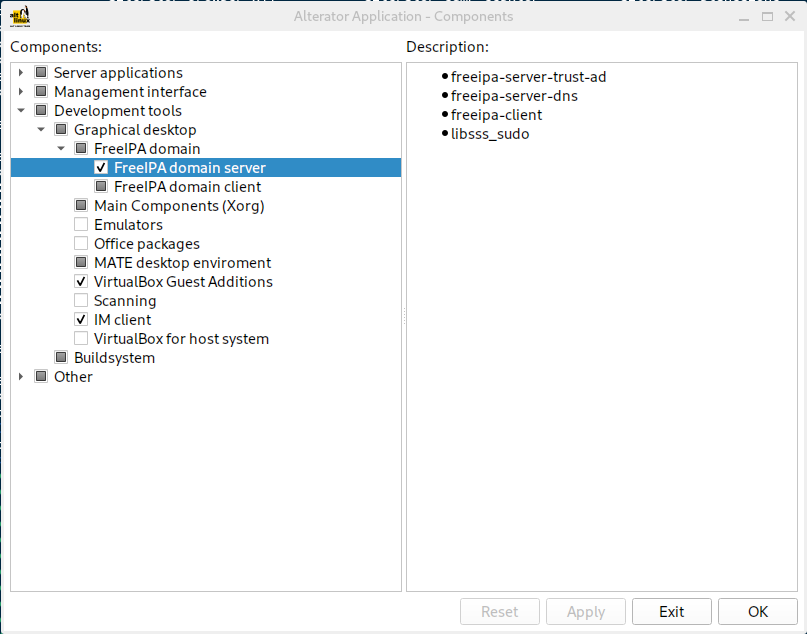
\includegraphics[width=10cm]{ierarchy.png}
	\caption{\label{fig_1}%
	Иерархия компонентов alterator-application-components}
\end{figure}

Демонстрация изменения состояния модели и её представления на рисунке \ref{fig_2}.

\begin{figure}[!ht]
	\centering
	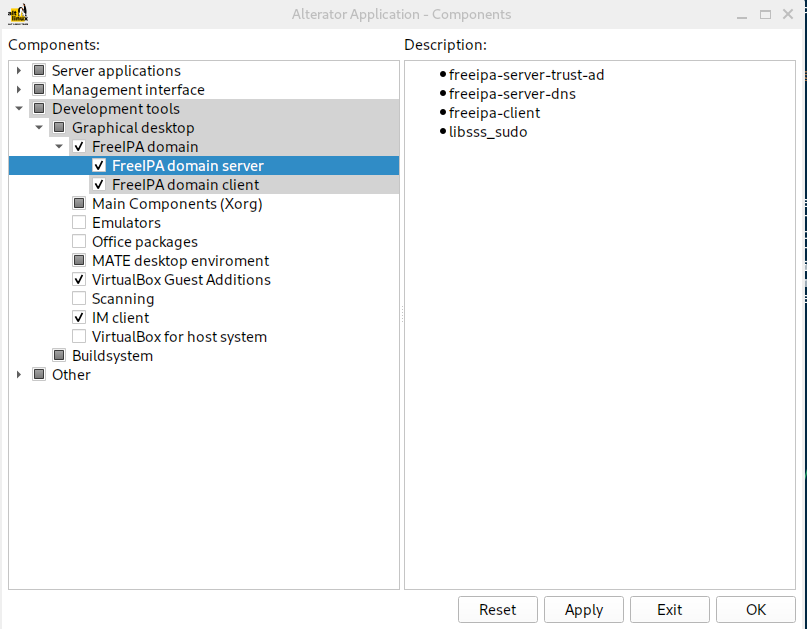
\includegraphics[width=10cm]{ierarchy-changed.png}
	\caption{\label{fig_2}%
	Изменение состояния модели}
\end{figure}

\newpage

% Раздел "Заключение"
\conclusion

Подводя итоги, мы ознакомились с разработкой и пакетированием приложений в семействе дистрибутивов ALT Linux.

В ходе работы в проект alterator-application-components была добавлена поддержка вложенных категорий.
Это должно сделать использование приложения конфигурирования ОС более удобным для пользователей, которыми, в частности, являются системные администраторы.

На текущий момент изменения, проделанные в данной работе, зафиксированы в релизе под номером 0.1.1-alt1 в репозитории Sisyphus.

%Библиографический список, составленный вручную, без использования BibTeX
%
%\begin{thebibliography}{99}
%  \bibitem{Ione} Источник 1.
%  \bibitem{Itwo} Источник 2
%\end{thebibliography}

%Библиографический список, составленный с помощью BibTeX

\inputencoding{cp1251}
\bibliographystyle{gost780uv}
\bibliography{thesis}
\inputencoding{utf8}

% Окончание основного документа и начало приложений
% Каждая последующая секция документа будет являться приложением
\appendix

\section{SPEC-файл smlnj}\label{spec}

\begin{Verbatim}[fontsize=\small,breaklines=true,numbers=left] 
Name: smlnj
Version: 2024.1
Release: alt1

Summary: The Standard ML of New Jersey Programming Language
License: BSD-3-Clause
Group: Development/Other
Url: https://github.com/smlnj/smlnj

BuildRequires: python3 cmake gcc gcc-c++

Source: %name-%version.tar
Patch: %name-alt-cfg.patch 

%description
Standard ML of New Jersey (abbreviated SML/NJ) is a compiler for the Standard ML '97 programming language with associated libraries, tools, and documentation. SML/NJ is free, open source software.

%prep
%setup -q
%patch0 -p1

%build
./build.sh

%install
mkdir -p %buildroot%_bindir
mkdir -p %buildroot%_libexecdir/%name
install -m 755 -D bin/* %buildroot%_bindir
install -m 755 -D bin/.arch-n-opsys %buildroot%_bindir
install -m 755 -D bin/.run-sml %buildroot%_bindir
install -m 755 -D bin/.link-sml %buildroot%_bindir
cp -r lib %buildroot%_libexecdir/%name/

%files
%dir %_libexecdir/%name
%_bindir/*
%_libexecdir/%name/*

%changelog
* Wed Jul 3 2024 Kirill Sharov <sheriffkorov@altlinux.org> 2024.1-alt1
- Initial release for Sisyphus.
\end{Verbatim}

\section{Diff-патч для smlnj}\label{patch}

\begin{Verbatim}[fontsize=\small,breaklines=true,numbers=left]
Binary files smlnj/.git/index and smlnj-changed/.git/index differ
diff -ur smlnj/runtime/c-libs/codegen/src/cfg.cxx smlnj-changed/runtime/c-libs/codegen/src/cfg.cxx
---- smlnj/runtime/c-libs/codegen/src/cfg.cxx	2024-07-02 13:54:59.549946281 +0400
+++ smlnj-changed/runtime/c-libs/codegen/src/cfg.cxx	2024-07-03 14:19:48.640069436 +0400
@@ -4,7 +4,7 @@
 //
 
 #include "cfg.hxx"
-
+#pragma GCC diagnostic ignored "-Wreturn-type"
 namespace CTypes {
     c_type * c_type::read (asdl::instream & is)
     {
diff -ur smlnj/runtime/c-libs/codegen/src/cfg-prim-codegen.cxx smlnj-changed/runtime/c-libs/codegen/src/cfg-prim-codegen.cxx
---- smlnj/runtime/c-libs/codegen/src/cfg-prim-codegen.cxx	2024-07-02 13:54:59.549946281 +0400
+++ smlnj-changed/runtime/c-libs/codegen/src/cfg-prim-codegen.cxx	2024-07-03 14:19:44.757071614 +0400
@@ -11,7 +11,7 @@
 
 #include "cfg.hxx"
 #include "target-info.hxx"
-
+#pragma GCC diagnostic ignored "-Wreturn-type"
 namespace CFG_Prim {
 
   // helper function to get LLVM type for numbers
\end{Verbatim}

\section{Квадратичная версия метода построения модели}\label{oldbuild}

\begin{Verbatim}[fontsize=\small,breaklines=true,numbers=left]
void ModelBuilder::build(Model *model)
{
    std::vector<std::unique_ptr<ComponentCategory>> categories = buildCategories();
    std::vector<std::unique_ptr<ComponentObject>> components   = buildObjects();
    for (auto &category : categories)
    {
        QString categoryId = category->m_id;
        auto categoryItem  = std::make_unique<ModelItem>(std::move(category));
        for (int i = 0; i < components.size(); ++i)
        {
            if (components[i]->m_category != categoryId)
                continue;
            auto componentItem = std::make_unique<ModelItem>(std::move(components[i]));
            categoryItem->insertRow(categoryItem->rowCount(), componentItem.release());
            components.erase(components.begin() + i);
        }
        // NOTE(cherniginma): don't add empty categories
        if (categoryItem->rowCount() != 0)
            model->insertRow(model->rowCount(), categoryItem.release());
    }

    if (components.empty())
        return;

    // NOTE(cherniginma): put the rest of components in default category
    auto defaultCategory = std::make_unique<ModelItem>(std::move(buildDefaultCategory()));
    for (auto &component : components)
    {
        auto componentItem = std::make_unique<ModelItem>(std::move(component));
        defaultCategory->insertRow(defaultCategory->rowCount(), componentItem.release());
    }
    model->insertRow(model->rowCount(), defaultCategory.release());

    model->correctCheckItemStates();
}

\end{Verbatim}

\section{Рекурсивная версия метода построения модели}\label{newbuild}

\begin{Verbatim}[fontsize=\small,breaklines=true,numbers=left]
void ModelBuilder::build(Model *model)
{
    auto categories = buildCategories();
    auto components = buildObjects();
    const QString &WITHOUT_PARENT{};
    for (auto &category : categories[WITHOUT_PARENT])
    {
        auto categoryItem = std::make_unique<ModelItem>(std::move(category));
        buildInner(dynamic_cast<ModelItem *>(categoryItem.get()), categories, components);
        if (categoryItem->rowCount())
            model->insertRow(model->rowCount(), categoryItem.release());
    }
    // NOTE(cherniginma): put the rest of components in default category
    auto defaultCategory = std::make_unique<ModelItem>(std::move(buildDefaultCategory()));
    for (auto &component : components[WITHOUT_PARENT])
    {
        auto componentItem = std::make_unique<ModelItem>(std::move(component));
        defaultCategory->insertRow(defaultCategory->rowCount(), componentItem.release());
    }
    // NOTE:(sharovkv) move the components from undefined categories to default category
    for (auto &[key, vec] : components)
    {
        if (categories.find(key) == categories.end())
        {
            for (auto &component : vec)
            {
                auto componentItem = std::make_unique<ModelItem>(std::move(component));
                defaultCategory->insertRow(defaultCategory->rowCount(), componentItem.release());
            }
        }
    }
    model->insertRow(model->rowCount(), defaultCategory.release());
    model->correctCheckItemStates();
}
\end{Verbatim}

\section{Квадратичная версия setCurrentState}\label{setcurrentstate}

\begin{Verbatim}[fontsize=\small,breaklines=true,numbers=left]
void Model::setCurrentState(ComponentsState state)
{
    for (int i = 0; i < rowCount(); i++)
    {
        auto categoryItem = dynamic_cast<ModelItem *>(invisibleRootItem()->child(i));
        for (int j = 0; j < categoryItem->rowCount(); j++)
        {
            auto componentItem = dynamic_cast<ModelItem *>(categoryItem->child(j));

            auto component = componentItem->data().value<ComponentObject *>();
            if (component)
            {
                const auto componentState = state[component->m_id];
                switch (componentState)
                {
                case ComponentState::installed:
                    setData(componentItem->index(), Qt::Checked, Qt::CheckStateRole);
                    break;
                case ComponentState::partially_installed:
                    setData(componentItem->index(), Qt::PartiallyChecked, Qt::CheckStateRole);
                    break;
                case ComponentState::not_installed:
                    setData(componentItem->index(), Qt::Unchecked, Qt::CheckStateRole);
                    break;
                }
            }
        }
    }
}
\end{Verbatim}

\section{Реализация resetCurrentStateInner}\label{resetcurrentstateinner}

\begin{Verbatim}[fontsize=\small,breaklines=true,numbers=left]
Qt::CheckState Model::resetCurrentStateInner(ModelItem *parent, ComponentsState &state)
{
    std::map<Qt::CheckState, int> hasVariant = {{Qt::Unchecked, 0}, {Qt::PartiallyChecked, 0}, {Qt::Checked, 0}};
    parent->setBackground(QColorConstants::White);
    const size_t numberOfChildren = parent->rowCount();
    for (size_t i = 0; i < numberOfChildren; ++i)
    {
        auto childItem = dynamic_cast<ModelItem *>(parent->child(i));
        if (childItem->itemType == ModelItem::Type::Category)
        {
            auto checkStateOfCategory = resetCurrentStateInner(childItem, state);
            childItem->setData(checkStateOfCategory, Qt::CheckStateRole);
            ++hasVariant[checkStateOfCategory];
        }
        else
        {
            auto component = childItem->data().value<ComponentObject *>();
            if (component)
            {
                auto checkStateOfComponent = static_cast<Qt::CheckState>(state[component->m_id]); 
                childItem->setData(checkStateOfComponent, Qt::CheckStateRole);
                ++hasVariant[checkStateOfComponent];
            }
        }
    }

    if (hasVariant[Qt::Unchecked] == numberOfChildren)
    {
        return Qt::Unchecked;
    }
    else if (hasVariant[Qt::Checked] == numberOfChildren)
    {
        return Qt::Checked;
    }
    return Qt::PartiallyChecked;
}
\end{Verbatim}

\end{document}
